\documentclass[10pt, a4paper]{article}
\usepackage[russian, english]{babel}
\usepackage{scn}
\usepackage{CJKutf8}
\usepackage{amsmath}
\usepackage[utf8]{inputenc}
\usepackage{cmap}
\usepackage{multicol} 
\usepackage{setspace} %межстрочный интервал
\usepackage{ragged2e}% выравнивания текста по ширине в документе.
\usepackage{fancyhdr} %настройки верхнего и нижнего колонтитулов в документе.
\usepackage{titlesec} %стилей заголовков разделов в документе.
\usepackage{enumitem} %настройки списков в документе.
\usepackage {graphicx}%Вставка картинок 
\usepackage[centercaption]{sidecap}
\usepackage{subfigure}
\usepackage{float}%"Плавающие" картинки
\usepackage{wrapfig}%Обтекание фигур (таблиц, картинок и прочего)
\usepackage[left=1.9cm,right=1.9cm, top=1cm,bottom=2.5cm]{geometry}
\justifying % выравнивает текст по ширине.
\fancyhf{} %очищает все верхние и нижние колонтитулы.
\renewcommand{\headrulewidth}{0pt} % remove the header rule
\cfoot{\vskip -1.5cm \thepage} %устанавливает номер страницы в нижнем колонтитуле.
\linespread{0.9} %устанавливает межстрочный интервал 
\setlength{\columnsep}{0.5cm}
\setcounter{page}{246}
\renewcommand{\thesection}{\Roman{section}} %устанавливает стиль нумерации разделов в виде заглавных римских цифр.
\titleformat{\section}{\footnotesize\centering\sc}{\thesection.}{0cm}{}[] %настраивает стиль заголовков разделов.
\newcommand{\RomanNumeralCaps}[1]
    {\MakeUppercase{\romannumeral #1}}



\begin{document}
\begin{SCn}
\begin{small}
\begin{multicols}{2}
\fontsize {10}{14}\selectfont 
\noindent
interpretation platform with a semantic model of the
system itself described in SC-code, encompassing submodels for the knowledge base, interfaces, and problem
solvers. A detailed description follows:\par
\vspace {0.5cm}
\noindent
\textit{A. Development of the Solver and Knowledge Base.}
\par
indent  The introduction of SC-code by OSTIS technology serves as a universal language for semantic expression of information in intelligent computing systems. It employs set theory for defining semantic aspects and graph theory for constructing syntactic structures, ensuring compatibility across different types of knowledge through semantic
memory (sc-memory). This approach not only simplifies
the description of various types of knowledge and models
but also allows for the construction of an ontological
model (sc-model) of any entity based on SC-code.
Developing a problem solver and knowledge base, especially for Alzheimer’s disease using OSTIS technology,
involves several key steps:
\begin{flushright}
\begin{enumerate}
\item [a)] Knowledge Representation: This step involves defining knowledge about Alzheimer’s disease, such as symptoms, diagnostic criteria, etc., and how this knowledge is represented within the OSTIS framework. The method of representation includes creating a semantic network to model the relationships
and entities related to Alzheimer’s disease.
 \vspace{-0.2cm}
\item [b)] Data Collection and Organization: Gathering and
documenting data, where the structure of the data
must be consistent with the chosen method of knowledge representation.
\vspace{-0.2cm}
\item [c)] Knowledge Base Development: Importing data into
the OSTIS system to establish a knowledge base,
which may include concepts, predicates, and rules
for controlling the logic of diagnosing Alzheimer’s
disease within the system.
\vspace{-0.2cm}
\item [d)] Solver Implementation: Developing the solver involves creating algorithms that can navigate the
knowledge base to provide diagnoses based on input
data. This includes implementing reasoning mechanisms that can assess patient data against the knowledge base to identify the presence of Alzheimer’s
disease.
\vspace{-0.2cm}
\item [e)] Data Storage: In compliance with medical data
storage regulations, the system needs not only to
possess a static knowledge base but also to have
the capability to store dynamic data such as patient
records and diagnostic results.
\vspace{-0.2cm}
\end{enumerate}
\end{flushright}
The semantic knowledge base is the cornerstone of
semantic communication, forming the foundational part
of the decision-making system. The data it contains
are authoritative, referential, and diverse. For different
domains, the objects encompassed by the knowledge base
vary, aiming to integrate scattered knowledge within the
domain, including historical data, real-time data, statistical analysis results, predictive models, as well as expert
knowledge and experience. Through computer technology, originally scattered knowledge is recombined and stored in different locations, enabling decision-makers to quickly access relevant information and resources.\par
 In application, the development of the knowledge base is primarily based on the information extracted, combined with the OSTIS framework, to construct a knowledge graph. This graph is further processed and refined to form a structured knowledge base. Storing semantically linked data about neurological diseases, it provides the necessary knowledge support for disease prediction.\par
\noindent
\scnheader{System Knowledge Base}\par
\noindent
$\supset$ \hspace{0.3cm} \textit {Declarative Knowledge} \par
\textit { \hspace{0.6cm} $\ni$ \hspace{0.3cm} Alzheimer’s Recognition Theory Concept
Ontology\\
$\supset$ \hspace{0.3cm} Procedural Knowledge}\par
\textit { \hspace{0.6cm} $\supset$ \hspace{0.3cm} System Knowledge}\par
\vspace{-0.1cm}

\hspace{1.2cm}  \begin{scnrelfromset} {splitting*:}
 \scnitem{  Model Building Knowledge}
 \scnitem{  Model Optimization Knowledge}
 \scnitem{   Results Display Knowledge}
\vspace{-0.3cm}
 \end{scnrelfromset}
\hspace{0.6cm} $\supset$ \hspace{0.3cm} \textit { Static Knowledge}\par
\hspace{1cm} $\ni$ \hspace{0.3cm} \textit {System Process}\par
\hspace{0.6cm} $\supset$ \hspace{0.3cm} \textit {Dynamic Knowledge}\par
\hspace{1cm} $\ni$ \hspace{0.3cm} \textit {Conditional Response in Specific Situations} \par
\vspace{0.2cm}
The problem solver performs basic actions of directly
modifying and managing the knowledge base, offering
a more dynamic component compared to the knowledge
base itself. It handles information stored in the knowledge
base to address specific problems, applying algorithms,
rules, and reasoning techniques to interpret, analyze, and
derive conclusions or solutions from available knowledge,
making decisions or generating new knowledge. Semantically, these operations are considered actions performed
within the memory of the acting entity, typically the
OSTIS system itself, with the knowledge base viewed
as its memory. Actions are executed based on the set
problem, describing the internal state of the intelligent
system or the required state of the external environment
for different problem categories.\par
Figure  \ref{fig:ss1.png} presents the SCG-code description of the
speech classification task within the set-theoretical ontology.\par
Within the OSTIS Technology framework, to achieve
the task of natural language processing, a specialized
ostis-system can be developed. The sc-model of the
problem solver is developed as a hierarchical system of
agents (sc-agents), providing flexibility and modularity
for the developed sc-agents. Abstract sc-agents are func
\end{multicols}
\newpage
\begin{multicols}{2}
\fontsize {10}{13}\selectfont
\vspace{-0.7cm}
\setcounter{figure}{1}
\begin{figure}[H]
\centering
 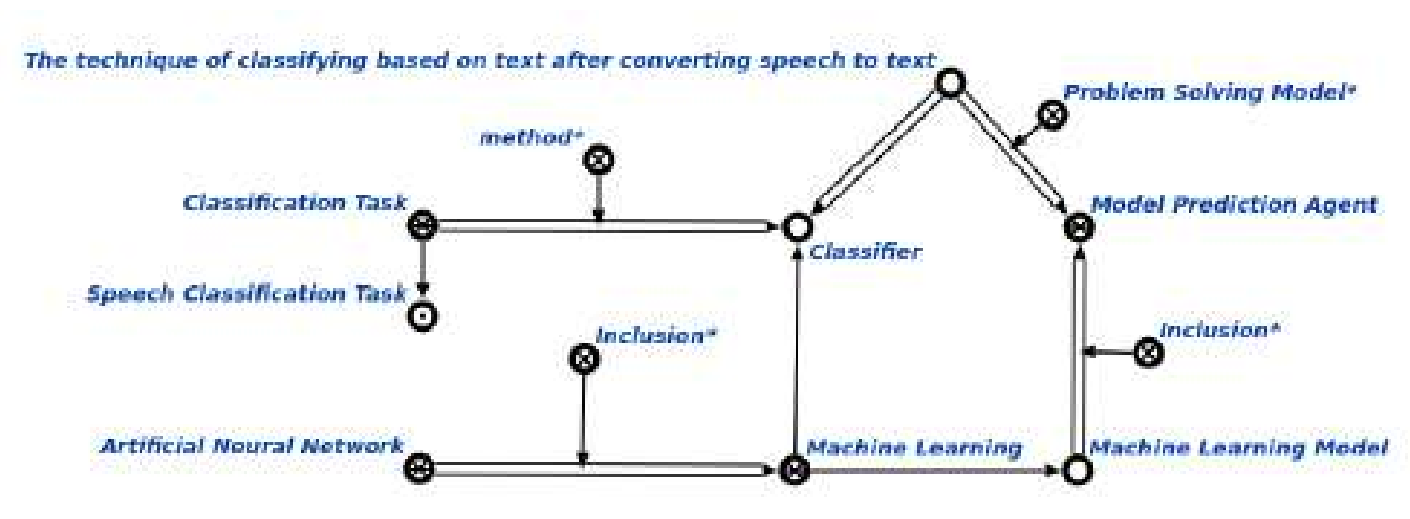
\includegraphics[width=0.9\linewidth]{ss1.png}
 \caption{\small A fragment of the set-theoretic ontology for speech classification tasks.}
  \label{fig:ss1.png}
\end{figure}
\noindent
tionally equivalent sc-agents of a certain category, with
different instances implemented in various programming
languages to address specific problems. In our work,
to implement an intelligent IT diagnostic system for
Alzheimer’s disease integrated with OSTIS, converting
natural language speech into diagnostic indicators required describing the entire process of natural language
processing and building extraction rules. Since in the
OSTIS technology framework, every action internally
represents some transformation executed by a specific
sc-agent (or a group of sc-agents), we consider the scmodel of the problem solver. The entire data processing
workflow is a core component of the system, ensuring efficient and accurate collection, transmission, processing,
and storage of data. An example of processing users’ data
within the system is shown in Figure  \ref{fig:ss2.png}.\\
\vspace{-0.1cm}
\setcounter{figure}{2}
\begin{figure}[H]
\centering
 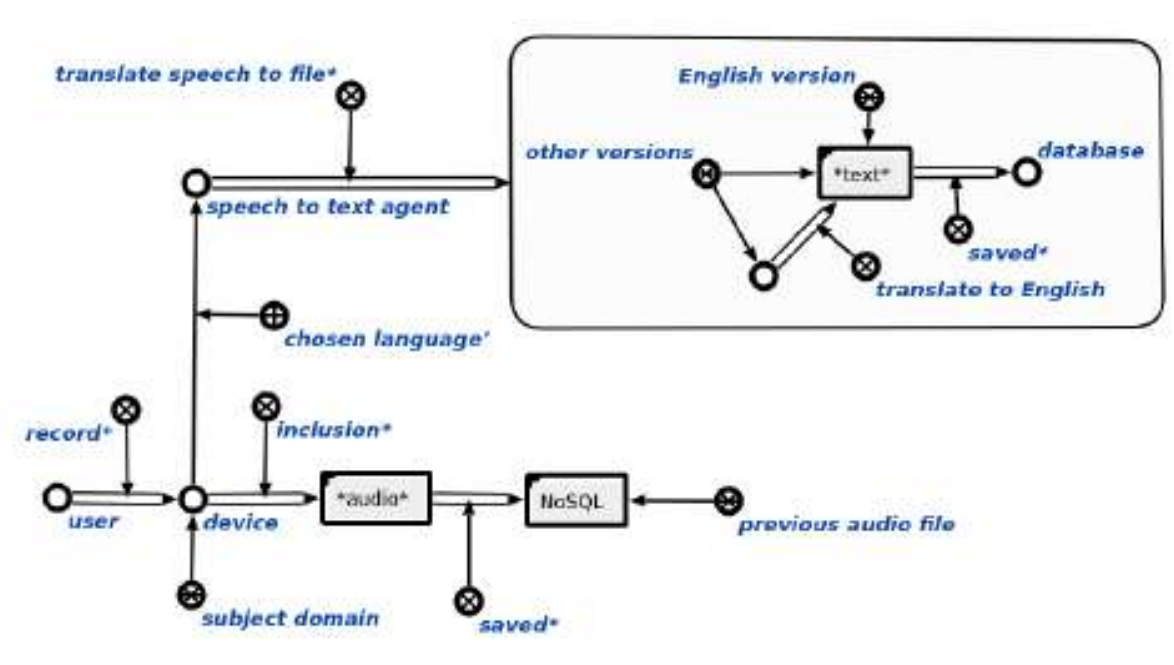
\includegraphics[width=1\linewidth]{ss2.png}
 \caption{\small An example of processing users’ data within the system.}
 \label{fig:ss2.png} 
 \end{figure}
\vspace{0.3cm}
\textit {B. Designing the User interface.}\\
Designing the user interface for the diagnostics system
requires careful consideration of the end-users, typically
healthcare professionals and possibly patients or their
families. The interface should be intuitive and facilitate
easy navigation through the diagnostic process:
\vspace{-0.2cm}
\begin{enumerate}
\item [1)] Information Input: Designing forms and input fields
that allow for easy entry of patient data and symptoms.
\vspace{-0.2cm}
\item [2)] Diagnostic Process Visualization: Providing visual
cues or progress indicators that guide the user
through the diagnostic process, helping them under
stand what stage the diagnosis is at and what steps
are next.
\vspace{-0.2cm}
\item [3)] Results Presentation: Displaying the diagnostic results in a clear, understandable format. This could
include a summary of findings, confidence levels,
and recommendations for further actions or treatments.
\end{enumerate}
Due to the use of component approach, the development of the entire natural language interface comes down
to development and improvement of separate specified
components (e.g. knowledge base on natural language
processing, component for natural language texts generation). The model of the process of responding to user
needs and the components of inference engine was shown
in figure \ref{fig:ss3.png}.\\
\vspace{-0.45cm}
\setcounter{figure}{3}
\begin{figure}[H]
\centering
 \includegraphics[width=1\linewidth]{ss3.png}
 \caption{\small The model of the process of responding to user needs.}
 \label{fig:ss3.png}
\end{figure}
The user interface includes all the components required for user interaction and obtaining results. The
general process of interacting with the user interface can
be described as follows:
\begin{itemize}
\item  The user reads all the necessary instructions.
\vspace{-0.2cm}
\item The user begins to record voice data according to
the instructions.
\vspace{-0.2cm}
\item The user ends the recording action and uploads the
data.
\vspace{-0.2cm}
\item The user presses the "Predict Data" button to receive
the probability of illness corresponding to their
voice data.
\vspace{-0.2cm}
\item The result is displayed in the result feedback area.
\end{itemize}
\indent
In the design of the user interface, taking the collection
of voice data as an example, the client-side page allows
participants to select from three functions: recording
voice information, converting voice to text, and predicting outcomes. The voice-to-text conversion serves as an
illustrative example of one method of data preprocessing.
Developers may adapt or modify this functionality based
on specific design requirements. After participants have
reco
In the report, the authors present an approach to
the design of an Internet of Things-based diagnostic
network aimed at using the OSTIS platform to expand the
possibilities of data interpretation within the intelligent
process of diagnosing Alzheimer’s disease. The structure
of the ontology for the description of the subject arearded their voice information onto their phones, the
device will save this voice data and carry out data preprocessing and feature extraction tasks. Upon activation
of the "predict" function by the participant, the phone,
acting as a client, will transmit the generated feature file
to the server. Following the receipt of prediction results
\end{multicols}
\newpage
\begin{multicols}{2}
\noindent  
sent from the server or another agent, the phone will
interpret these results and display them on the page.
User interface design is based on a component-based
approach, any user interface component can be described
in the ostis-system knowledge base. An illustration of the
user interface displaying the probability of a participant
being diagnosed with Alzheimer’s disease is presented
in Figure \ref{fig:ss4.png}.\\
\vspace{-0.2cm}
\setcounter{figure}{4}
\begin{figure}[H]
\centering
 \includegraphics[width=1\linewidth]{ss4.png}
 \caption{\small An example of the user interface}
 \label{fig:ss4.png}
\end{figure}
For the corresponding SCg-code description fragment
within the OSTIS system knowledge base, see Figure \ref{fig:ss5.png}.
\vspace{-0.45cm}
\setcounter{figure}{5}
\begin{figure}[H]
\centering
 \includegraphics[width=1\linewidth]{ss5.png}
 \caption{\small SCg-code of the user interface.}
 \label{fig:ss5.png}
\end{figure}
\begin{center}
\RomanNumeralCaps{6} Conclusion and future works
\end{center} \\
In the report, the authors present an approach to
the design of an Internet of Things-based diagnostic
network aimed at using the OSTIS platform to expand the
possibilities of data interpretation within the intelligent
process of diagnosing Alzheimer’s disease. The structure
of the ontology for the description of the subject area
is given. The process of developing solvers, knowledge
bases and user interfaces adapted for healthcare professionals and patients is described taking into account the
stages from data collection to presentation of diagnostic
results. In the future, the work will focus on improving
the OSTIS-based OTNET to increase the accuracy of
recognition and study its applicability to the treatment
process, thereby expanding the possibilities of intelligent
diagnostics in the field of medicine.\par
\vspace{-0.1cm}
\begin{center}
References
\end{center}
\vspace{-0.3cm}
\footnotesize
\begin{enumerate}
    \item [[1]] T. Shuo, Y. Wenbo, L. G. Jehane Michael, W. Peng, H. Wei,
and Y. Zhewei, “Smart healthcare: making medical care more
intelligent,” Global Health Journal, vol. 3, no. 3, pp. 62–65, 2019.
\vspace{-0.19cm}
\item [[2]]J. Zhang, Y. Li, L. Cao, and Y. Zhang, “Research on the
construction of smart hospitals at home and abroad,” Chinese
Hospital Management, vol. 38, pp. 64–66, 2018.
\vspace{-0.19cm}
\item [[3]]K. Clemens Scott and B. Amanda, “Health information technology continues to show positive effect on medical outcomes:
systematic review,” Journal of medical Internet research, vol. 20,
no. 2, 2018, article e41.
\vspace{-0.19cm}
\item [[4]] B. Pradhan, S. Bhattacharyya, and K. Pal, “Iot-based applications
in healthcare devices,” Journal of healthcare engineering, vol.
2021, pp. 1–18, 2021, article ID 6632599.
\vspace{-0.45cm}
 \item [[5]] (2020) Alzheimer disease relevance ontology by process.
[Online]. Available: https://bioportal.bioontology.org/ontologies/
AD-DROP/?p=classesconceptid=root
\vspace{-0.19cm}
\item [[6]]  G. Szatloczki, I. Hoffmann, V. Vincze, J. Kalman, and M. Pakaski,
“Speaking in alzheimer’s disease, is that an early sign? importance
of changes in language abilities in alzheimer’s disease,” Frontiers
in aging neuroscience, vol. 7, 2015, article 195.
\vspace{-0.19cm}
\item [[7]] F. Martínez-Sánchez, J. J. G. Meilán, J. Carro, and O. Ivanova, “A
prototype for the voice analysis diagnosis of alzheimer’s disease,”
Journal of Alzheimer’s disease, vol. 64, no. 2, pp. 473–481, 2018.
\vspace{-0.1cm}
\item [[8]] R. D. Nebes, C. B. Brady, and F. J. Huff, “Automatic and attentional mechanisms of semantic priming in alzheimer’s disease,”
Journal of Clinical and Experimental Neuropsychology, vol. 11,
no. 2, pp. 219–230, 1989.
\vspace{-0.2cm}
\item [[9]] A. Satt, R. Hoory, A. König, P. Aalten, and P. H. Robert, “Speechbased automatic and robust detection of very early dementia,” in
Fifteenth Annual Conference of the International Speech Communication Association, 2014, p. 2538––2542.
\vspace{-0.19cm}
\item [[10]] U. Vishniakou and C. Yu, “Using machine learning for recognition of Alzheimer’s disease based on transcription information,”
\end{enumerate}
Reports of BSUIR, vol. 21, no. 6, pp. 106–112, 2023.\\
\selectlanguage{russian}
\begin{center}
    

\large
\textbf{РАЗРАБОТКА СЕТИ ИНТЕРНЕТА ВЕЩЕЙ ДЛЯ ДИАГНОСТИКИ БОЛЕЗНИ АЛЬЦГЕЙМЕРА С ИСПОЛЬЗОВАНИЕМ OSTIS}\\
\normalsize
Вишняков В.А., Чуюэ Юй
\end{center}\\
\indent
Доклад посвящен разработке Интернета вещей для диагностики болезни Альцгеймера (БА) с использованием
технологии OSTIS. Приведена структура онтологии для
описания элементов заболевания БА. В статье рассматривается построение ИТ-диагностической сети БА, использующей семантические возможности платформы OSTIS для
обработки и анализа медицинских данных. Представлены
элементы описания базы знаний, решателей и пользовательского интерфейса с использованием компонентного подхода
к проектированию.\\
\indent
Ключевые слова: сеть интернета вещей, болезнь Альцгеймера, база знаний, решатель, пользовательский интерфейс,
ИТ-диагностика, OSTIS.\\
\begin{flushright}
Received 31.03.2024
\end{flushright}
\end{multicols}
\end{small}
\end{SCn}
\end{document}
